%%%%%%%%%%%%%%%%%%%%%%%%%%%%%%%%%%%%%%%%%
% University Assignment Title Page 
% LaTeX Template
% Version 1.0 (27/12/12)
%
% This template has been downloaded from:
% http://www.LaTeXTemplates.com
%
% Original author:
% WikiBooks (http://en.wikibooks.org/wiki/LaTeX/Title_Creation)
%
% License:
% CC BY-NC-SA 3.0 (http://creativecommons.org/licenses/by-nc-sa/3.0/)
% 
% Instructions for using this template:
% This title page is capable of being compiled as is. This is not useful for 
% including it in another document. To do this, you have two options: 
%
% 1) Copy/paste everything between \begin{document} and \end{document} 
% starting at \begin{titlepage} and paste this into another LaTeX file where you 
% want your title page.
% OR
% 2) Remove everything outside the \begin{titlepage} and \end{titlepage} and 
% move this file to the same directory as the LaTeX file you wish to add it to. 
% Then add \input{./title_page_1.tex} to your LaTeX file where you want your
% title page.
%
%%%%%%%%%%%%%%%%%%%%%%%%%%%%%%%%%%%%%%%%%
%\title{Title page with logo}
%----------------------------------------------------------------------------------------
%   PACKAGES AND OTHER DOCUMENT CONFIGURATIONS
%----------------------------------------------------------------------------------------

\documentclass[12pt]{article}
\usepackage[english]{babel}
\usepackage[utf8x]{inputenc}
\usepackage{amsmath}
\usepackage{graphicx}
\usepackage[colorinlistoftodos]{todonotes}

\begin{document}

\begin{titlepage}

\newcommand{\HRule}{\rule{\linewidth}{0.5mm}} % Defines a new command for the horizontal lines, change thickness here

\center % Center everything on the page
 
%----------------------------------------------------------------------------------------
%   HEADING SECTIONS
%----------------------------------------------------------------------------------------

\textsc{\LARGE Dalhousie University}\\[1.5cm] % Name of your university/college
\textsc{\Large Topics in Program Comprehension}\\[0.5cm] % Major heading such as course name
\textsc{\large CSCI 6306}\\[0.5cm] % Minor heading such as course title

%----------------------------------------------------------------------------------------
%   TITLE SECTION
%----------------------------------------------------------------------------------------

\HRule \\[0.4cm]
{ \huge \bfseries Architecture Extraction}\\[0.4cm] % Title of your document
\HRule \\[1.5cm]
 
%----------------------------------------------------------------------------------------
%   AUTHOR SECTION
%----------------------------------------------------------------------------------------

~
%\begin{minipage}{0.4\textwidth}
%\begin{flushright} \large
\emph{Group : Something} \\
Bhupendra \textsc{Rajawat} \\
Bryan Thomas \textsc{D'silva}\\ % Supervisor's Name 
Saurabh \textsc{Singh}\\
\bigskip
%\end{flushright}
%\end{minipage}\\[2cm]

% If you don't want a supervisor, uncomment the two lines below and remove the section above
%\Large \emph{Author:}\\
%John \textsc{Smith}\\[3cm] % Your name

%----------------------------------------------------------------------------------------
%   DATE SECTION
%----------------------------------------------------------------------------------------

{\large \today}\\[2cm] % Date, change the \today to a set date if you want to be precise

%----------------------------------------------------------------------------------------
%   LOGO SECTION
%----------------------------------------------------------------------------------------


\includegraphics[width=0.7\textwidth]{dal.jpg}% Include a department/university logo - this will require the graphicx package
 
%----------------------------------------------------------------------------------------

\vfill % Fill the rest of the page with whitespace

\end{titlepage}
\tableofcontents
\newpage
\begin{abstract}
Your abstract.
\end{abstract}

\section{Finding a Software System}
We looked at the following software systems and games.
\begin{enumerate}
\item \textbf{Kodi}: Kodi is an open source software media player and entertainment hub. This is available on atleast seven platforms. This was one of the first softwares we looked at and kept it as a contender

\item \textbf{Quake III}: The source code for Quake is challenging and interesting. However, there is almost no documentation for the same and hence we decided not to go ahead with this for now.

\item \textbf{GIMP}: GIMP is a cross platform image editor with an excellent community backing it up. We decided to extract the architecture for GIMP. We talk more about GIMP in the further sections.

\end{enumerate}

We also looked at Doom3, SuperTuxKart, Wordpress, TuxRunner and Linux but found GIMP to be the most interesting on to use for this assignment
\section{About GIMP}
\section{Counting the lines of code}
\subsection{Count Lines of Code}
Count Lines of Code, abbreviated as CLOC is a software used to count comment lines, blank lines and physical lines of code\cite{gitid}. We used this software initially when we looked at what software system we need to pick. We can look at figure \ref{fig:clocgimp} for the output for GIMP.
\begin{figure}
\centering
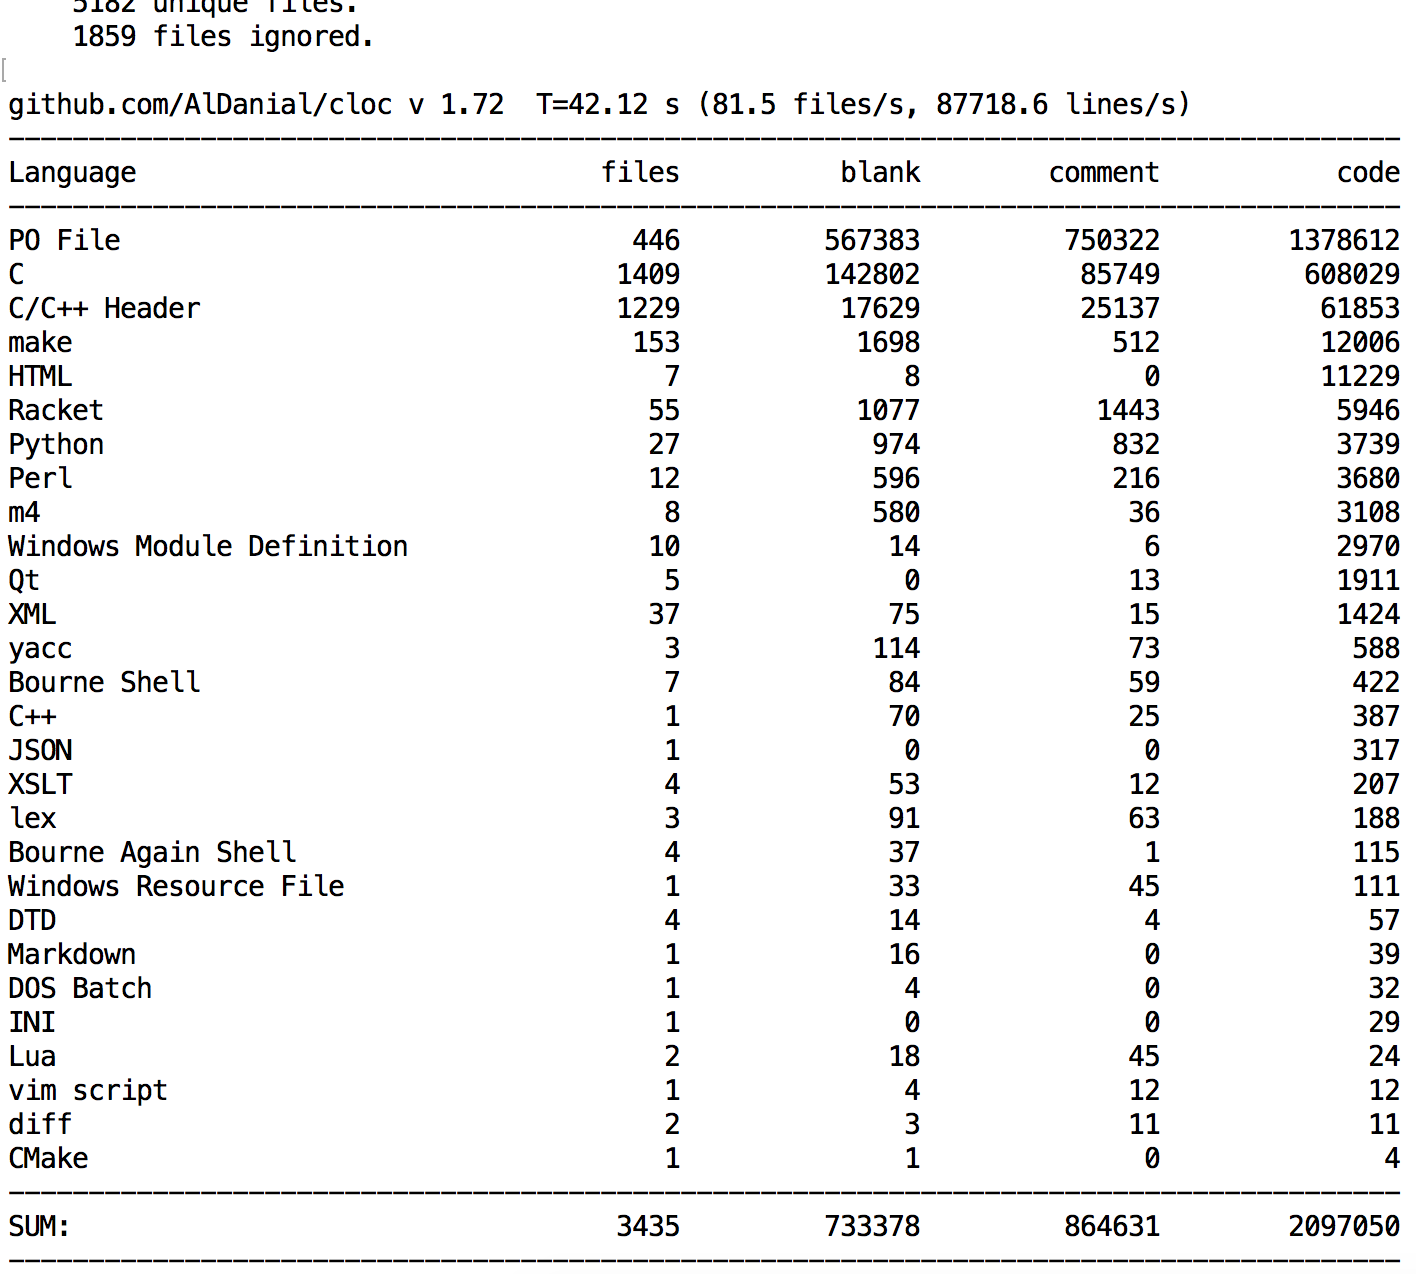
\includegraphics[width=1\textwidth]{clocgimp.png}
\caption{\label{fig:clocgimp}CLOC output for GIMP}
\end{figure}
%LocMetrics
\subsection{LocMetrics}
LocMetrics\cite{locmetrics} is very similar to what CLOC does. We did find this software interesting because of how it visualized the output.

\section{Directory Structure}
\section{Entry Point}
\section{Build Process}
\section{Control Flow}
\section{Dependencies}
\section{Functional Needs}
\section{Conclusion}

\subsection{Tables and Figures}

Use the table and tabular commands for basic tables --- see Table~\ref{tab:widgets}, for example. You can upload a figure (JPEG, PNG or PDF) using the files menu. To include it in your document, use the includegraphics command as in the code for Figure~\ref{fig:frog} below.


\begin{enumerate}
\item Like this,
\item and like this.
\end{enumerate}
\dots or bullet points \dots
\begin{itemize}
\item Like this,
\item and like this.
\end{itemize}

We hope you find write\LaTeX\ useful, and please let us know if you have any feedback using the help menu above.

\newpage
\begin{thebibliography}{9}
	\bibitem{cloc} 
	https://github.com/AlDanial/cloc
	
	\bibitem{LocMetrics}
	http://www.locmetrics.com/
	
\end{thebibliography}
\end{document}